 \documentclass[12pt, a4paper, oneside]{report}

% ============================================================
% Page Layout (per UE requirements: 2cm L, 4cm R, 2.5cm T, 3cm B)
% ============================================================
\usepackage[left=2cm, right=4cm, top=2.5cm, bottom=3cm]{geometry}

% ============================================================
% Font & Encoding
% ============================================================
\usepackage[T1]{fontenc}
\usepackage[utf8]{inputenc}
\usepackage{mathptmx}          % Times New Roman clone

% ============================================================
% Core Packages
% ============================================================
\usepackage{graphicx}           % Figures
\usepackage{booktabs}           % Professional tables
\usepackage{amsmath, amssymb}   % Math
\usepackage{hyperref}           % Clickable links
\usepackage{natbib}             % Harvard-style citations
\usepackage{setspace}           % Line spacing
\usepackage{parskip}            % Paragraph spacing
\usepackage{indentfirst}        % Indent first paragraph
\usepackage{float}              % Figure placement
\usepackage{caption}            % Caption formatting
\usepackage{enumitem}           % List customization
\usepackage{xcolor}             % Colors (for hyperref)
\usepackage{listings}           % Code listings
\usepackage{appendix}           % Appendix support
\usepackage{longtable}          % Multi-page tables
\usepackage{multirow}           % Table cell merging
\usepackage{pdflscape}          % Landscape pages
\usepackage{fancyhdr}           % Headers/footers

% ============================================================
% University Branding Colors (UE Germany Official)
% ============================================================
\definecolor{UERed}{HTML}{F9423A}          % UE primary red
\definecolor{UEDoveBlue}{HTML}{3C4554}     % UE secondary dove blue
\definecolor{UEGrey}{HTML}{64666A}         % UE cool grey

% ============================================================
% Formatting
% ============================================================
\setlength{\parindent}{1cm}     % 1cm paragraph indent (per UE)
\onehalfspacing                 % 1.5 line spacing

\hypersetup{
    colorlinks=true,
    linkcolor=black,
    citecolor=black,
    urlcolor=blue,
    pdfauthor={Mukhammadsidik Ibrokhimov},
    pdftitle={Comparing Machine Learning Methods for Predicting Diseases from Symptoms in Healthcare}
}

% Header/footer
\pagestyle{fancy}
\fancyhf{}
\fancyhead[R]{\thepage}
\renewcommand{\headrulewidth}{0pt}

% ============================================================
% Document Metadata
% ============================================================
\title{Comparing Machine Learning Methods for Predicting Diseases from Symptoms in Healthcare}
\author{Mukhammadsidik Ibrokhimov}
\date{\today}

% ============================================================
\begin{document}

% --- Cover Page ---
\begin{titlepage}
    % Top colored bar with UE logo
    \noindent
    \begin{minipage}{\textwidth}
        \colorbox{UERed}{%
            \begin{minipage}{\dimexpr\textwidth-2\fboxsep}
                \vspace{0.5cm}
                \centering
                {\color{white}\fontsize{40}{48}\selectfont\textbf{UE}}
                \vspace{0.3cm}
            \end{minipage}%
        }
    \end{minipage}

    \vspace{1.5cm}

    \centering

    % University name and faculty
    {\large\color{UEDoveBlue}\textbf{University of Europe for Applied Sciences}}\\[0.3cm]
    {\large\color{UEGrey}Faculty of Software Engineering}\\[0.5cm]

    % Decorative line
    {\color{UERed}\rule{0.7\textwidth}{2pt}}\\[1.5cm]

    % Thesis title
    {\LARGE\bfseries Comparing Machine Learning Methods for\\ Predicting Diseases from Symptoms in Healthcare}\\[1.5cm]

    % Decorative line
    {\color{UERed}\rule{0.5\textwidth}{1pt}}\\[1cm]

    % Degree information
    {\large Bachelor Thesis}\\[0.4cm]
    {\normalsize submitted in partial fulfillment of the requirements for the degree of}\\[0.4cm]
    {\large\bfseries Bachelor of Science (B.Sc.)}\\[0.3cm]
    {\normalsize in Software Engineering}\\[1.5cm]

    % Author and supervisor information
    \begin{flushleft}
        \hspace{3cm}
        \begin{tabular}{@{}ll}
            \textbf{Author:}             & Mukhammad Ibrokhimov \\[0.3cm]
            \textbf{Matriculation No:}   & [Your Matriculation Number] \\[0.3cm]
            \textbf{First Supervisor:}   & [Prof. Dr. First Supervisor] \\[0.3cm]
            \textbf{Second Supervisor:}  & [Second Supervisor] \\[0.3cm]
            \textbf{Date of Submission:} & \today \\
        \end{tabular}
    \end{flushleft}

    \vfill

    % Bottom section with location
    {\large Berlin, \today}

    \vspace{0.5cm}

    % Bottom accent line
    \noindent
    {\color{UERed}\rule{\textwidth}{3pt}}

\end{titlepage}


% --- Statement of Authorship ---
\chapter*{Statement of Authorship}
\addcontentsline{toc}{chapter}{Statement of Authorship}

\renewcommand{\arraystretch}{1.4}
\noindent
\begin{tabular}{@{}p{7.3cm} p{7.3cm}@{}}
\textbf{Family Name:} Ibrokhimov & \textbf{First Name:} Mukhammadsidik \\[0.3cm]
\textbf{Student ID:} 55094865 & \textbf{Title of Thesis:} Comparing Machine Learning Methods for Predicting Diseases from Symptoms in Healthcare \\
\end{tabular}

\vspace{0.8cm}

\noindent With my signature, I confirm to be the sole author of the thesis presented. Where the work of others has been consulted, this is duly acknowledged in the thesis' bibliography. All verbatim or referential use of the sources named in the bibliography has been specifically indicated in the text.

\vspace{0.4cm}

\noindent The thesis at hand has not been presented to another examination board. It has not been part of an assignment over my course of studies and has not been published. The paper version of this thesis is identical to the digital version handed in.

\vfill

\noindent
\begin{minipage}[t]{0.45\textwidth}
\rule{\textwidth}{0.4pt}\\
Berlin, \today\\[0.1cm]
{\small Date, Place}
\end{minipage}
\hfill
\begin{minipage}[t]{0.45\textwidth}
\rule{\textwidth}{0.4pt}\\
Mukhammadsidik Ibrokhimov\\[0.1cm]
{\small Signature}
\end{minipage}

\clearpage


% --- Declaration on AI Use ---
\chapter*{Declaration on the Use of Generative Artificial Intelligence (AI) Systems}
\addcontentsline{toc}{chapter}{Declaration on the Use of AI}

\renewcommand{\arraystretch}{1.4}
\noindent
\begin{tabular}{@{}p{7.3cm} p{7.3cm}@{}}
\textbf{Family Name:} Ibrokhimov & \textbf{First Name:} Mukhammadsidik \\[0.3cm]
\textbf{Student ID:} 55094865 & \textbf{Title of the Exam:} Comparing Machine Learning Methods for Predicting Diseases from Symptoms in Healthcare \\
\end{tabular}

\vspace{0.8cm}

\noindent I have used the following artificial intelligence (AI)-based tools in the creation of my work:

\begin{enumerate}[leftmargin=2cm, itemsep=0.1cm]
    \item ChatGPT (Version 4o / 5), OpenAI
    \item Claude (Sonnet 4.6 / Opus 4.6), Anthropic
    \item GitHub Copilot, GitHub / Microsoft
    \item Grammarly, Grammarly Inc.
\end{enumerate}

\vspace{0.4cm}

\noindent I further declare that
\begin{itemize}[label={$\boxtimes$}, leftmargin=2cm, itemsep=0.1cm]
    \item I have actively informed myself about the performance and limitations of the above-mentioned AI tools,
    \item I have marked the passages taken from the above-mentioned AI tools,
    \item I have checked that the content generated with the help of the above-mentioned AI tools and adopted by me is actually accurate,
    \item I am aware that, as the author of this work, I am responsible for the information and statements made in it.
\end{itemize}

\vspace{0.4cm}

\noindent I have used the AI-based tools mentioned above as shown in the table below.

\begin{table}[H]
\centering
\renewcommand{\arraystretch}{1.4}
\begin{tabular}{@{}p{3.0cm} p{4.2cm} p{3.6cm} p{2.6cm}@{}}
\toprule
\textbf{AI-based support tool} & \textbf{Usage} & \textbf{Parts of the work affected} & \textbf{Remarks} \\
\midrule
ChatGPT 4o / 5, OpenAI & Language editing, rephrasing my own draft text for clarity, and structural suggestions & All chapters (text refinement only) & Output reviewed and edited by the author \\
Claude Sonnet 4.6 / Opus 4.6, Anthropic & Language editing, brainstorming, and code-debugging assistance & All chapters; \texttt{experiments/} code & Output reviewed and edited by the author \\
GitHub Copilot & Code completion suggestions during implementation & \texttt{experiments/} source code only; not in thesis text & --- \\
Grammarly & Grammar, spelling, and style correction & All chapters & --- \\
\bottomrule
\end{tabular}
\end{table}

\vfill

\noindent
\begin{minipage}[t]{0.45\textwidth}
\rule{\textwidth}{0.4pt}\\
Berlin, \today\\[0.1cm]
{\small Place, Date}
\end{minipage}
\hfill
\begin{minipage}[t]{0.45\textwidth}
\rule{\textwidth}{0.4pt}\\
Mukhammadsidik Ibrokhimov\\[0.1cm]
{\small Signature of the Student}
\end{minipage}

\clearpage


% --- Front Matter ---
\pagenumbering{roman}
\tableofcontents
\listoffigures
\listoftables

% --- Abstract ---
\chapter*{Abstract}
\addcontentsline{toc}{chapter}{Abstract}

The identification of patient symptoms in time and correctly to enhance access to healthcare and decrease avoidable medical visits is relevant. I have compared five machine learning classifiers in this thesis (Naive Bayes, Logistic Regression, Support Vector Machine, Random Forest, and XGBoost) to predict diseases with a number of classes using binary symptom vectors. I compare them on two publicly available Kaggle datasets, a small dataset consisting of about 5,000 records with 132 symptoms and 41 diseases and a larger dataset consisting of about 246,000 records with a considerably larger set of classes. In the case of Dataset 1, I use stratified cross-validation using grid search. In Dataset 2, I apply fixed hyperparameters to make the experiments computationally feasible. I compare all models based on accuracy, precision, recall and F1-score to determine the approaches that are best to use in predicting symptoms. Limitations of the study are the lack of external clinical validation, binary representation of symptoms, and simplified one-disease formulation. Besides the metric findings, I address real-world trade-offs of interpretability, computational cost, and regulatory requirements on the EU AI Act and GDPR to actual healthcare booking systems.

\vspace{0.5cm}
\noindent\textbf{Keywords:} machine learning, disease prediction, symptom-based classification, healthcare, Random Forest, XGBoost, comparative study


% --- Main Content ---
\pagenumbering{arabic}
\setcounter{page}{1}

\chapter{Introduction}
\label{ch:introduction}

\section{Background and Motivation}
\label{sec:background}

The growing demand for healthcare services worldwide has placed significant pressure on medical systems, leading to long waiting times, delayed diagnoses, and inefficient resource allocation. According to the World Health Organization, timely access to appropriate healthcare remains a critical challenge, particularly in primary care settings where patients often struggle to identify the correct medical specialist for their symptoms \citep{WHO2021}. This challenge is compounded by the increasing complexity of diseases and the limited availability of general practitioners who can serve as effective gatekeepers in the referral process.

Machine learning has emerged as a promising approach to support clinical decision-making by leveraging large volumes of patient data to identify patterns that may not be immediately apparent to human practitioners \citep{Rajpurkar2022}. In particular, symptom-based disease prediction models have the potential to assist both patients and healthcare providers by offering preliminary assessments based on reported symptoms. Such models could serve as decision-support tools that help patients navigate the healthcare system more effectively, for instance by suggesting whether a visit to a general practitioner, a specialist, or an emergency department is most appropriate.

Several machine learning classifiers have been applied to the problem of disease prediction from symptoms, including traditional approaches such as Naive Bayes and Logistic Regression, as well as more recent ensemble methods like Random Forest and XGBoost \citep{Uddin2019}. However, the comparative performance of these methods on symptom-based datasets remains insufficiently explored in the literature, particularly when considering practical deployment scenarios where interpretability, computational efficiency, and robustness to class imbalance are important considerations.

\section{Problem Statement}
\label{sec:problem_statement}

Despite the availability of multiple machine learning algorithms suitable for multi-class classification tasks, there is a lack of systematic comparison of these methods specifically for symptom-based disease prediction. Existing studies often evaluate a single model or a narrow set of classifiers, making it difficult for practitioners to select the most appropriate approach for a given clinical context. Furthermore, many studies do not adequately address challenges such as class imbalance, which is inherent in medical datasets where some diseases are far more prevalent than others.

\section{Research Question}
\label{sec:research_question}

This thesis addresses the following research question:

\begin{quote}
\textit{How do Naive Bayes, Logistic Regression, Support Vector Machine, Random Forest, and XGBoost compare in terms of accuracy, precision, recall, and F1-score when applied to symptom-based disease prediction, and which method offers the best trade-off between predictive performance and practical applicability for healthcare decision support?}
\end{quote}

\section{Objectives}
\label{sec:objectives}

To answer this research question, the thesis pursues the following objectives:

\begin{enumerate}
    \item Conduct a literature review of machine learning approaches for symptom-based disease prediction, identifying current methods, datasets, and evaluation practices.
    \item Describe and preprocess two publicly available Kaggle datasets for symptom-based disease classification.
    \item Implement and train five machine learning classifiers --- Naive Bayes, Logistic Regression, Support Vector Machine, Random Forest, and XGBoost --- using consistent experimental conditions.
    \item Evaluate and compare the classifiers using standard metrics (accuracy, precision, recall, F1-score) and analyze error patterns through confusion matrices and feature importance analysis.
    \item Discuss the practical implications of the results for healthcare booking and triage decision support.
\end{enumerate}

\section{Scope and Limitations}
\label{sec:scope}

This thesis focuses exclusively on predicting disease categories from binary symptom vectors. It does not address specialist mapping, treatment recommendation, or real-time clinical deployment. The evaluation is limited to two publicly available datasets and does not involve clinical validation with real patient data. The implications for healthcare booking are discussed at a conceptual level rather than through a deployed system.

\section{Thesis Structure}
\label{sec:thesis_structure}

The remainder of this thesis is organized as follows. Chapter~\ref{ch:literature_review} reviews the relevant literature on machine learning in healthcare and symptom-based disease prediction. Chapter~\ref{ch:data_description} describes the two datasets used in this study and the preprocessing steps applied. Chapter~\ref{ch:methodology} presents the methodology, including the five classifiers, the handling of class imbalance, and the evaluation metrics. Chapter~\ref{ch:results} reports the experimental results. Chapter~\ref{ch:discussion} discusses the findings, limitations, and ethical considerations. Finally, Chapter~\ref{ch:conclusion} summarizes the contributions and outlines directions for future work.

\vspace{1cm}

\noindent\textbf{Thesis Statement:} This thesis demonstrates that ensemble methods, specifically Random Forest and XGBoost, consistently outperform traditional classifiers such as Naive Bayes, Logistic Regression, and Support Vector Machine for symptom-based disease prediction across two datasets of different scales. However, the choice of the most suitable model depends not only on predictive accuracy but also on practical considerations including interpretability, computational cost, and robustness to class imbalance, all of which are critical for real-world healthcare decision support.

\chapter{Literature Review}
\label{ch:literature_review}

This chapter covers the existing research on machine learning for disease prediction. I start with the general use of ML in healthcare, then narrow down to symptom-based prediction, discuss the main challenges, and end with the healthcare booking context that motivates this work.

\section{Machine Learning in Healthcare}
\label{sec:ml_healthcare}

Machine learning has been applied to healthcare for over a decade, but the field has accelerated with the digitization of medical records and cheaper computing power. \citet{Topol2019} provided an early overview of how AI is changing clinical practice, showing that ML models can match or exceed human performance in specific tasks like reading X-rays or pathology slides. \citet{Rajpurkar2022} later surveyed the broader landscape and pointed out that while image-based diagnosis has received most of the attention, structured clinical data --- such as symptom records --- remains underexplored.

In healthcare, the dominant ML approach is supervised classification: train a model on labeled examples (patient features + diagnosis) and use it to predict diagnoses for new patients. The classifiers used most often include Naive Bayes, Logistic Regression, SVM, Decision Trees, Random Forest, and XGBoost \citep{Uddin2019}. \citet{Sarker2021} provides a useful categorization of these methods.

\citet{Davenport2019} divided healthcare AI into three areas: clinical decision support, patient engagement, and administrative efficiency. Disease prediction falls into the first category. The key point is that these models are meant to assist doctors, not replace them. This means they need to be not just accurate but also interpretable and safe.

One thing that stood out to me while reading the literature is that accuracy alone is not a good enough metric for medical ML. \citet{Rajpurkar2022} argued that precision, recall, and AUC-ROC give a better picture, especially on imbalanced datasets where rare diseases can be completely missed by an accuracy-optimized model. This is why I adopted a multi-metric approach in my evaluation (Chapter~\ref{ch:results}).

\section{Symptom-Based Disease Prediction}
\label{sec:symptom_prediction}

Symptom-based disease prediction is a specific type of supervised classification where the inputs are patient-reported symptoms and the output is a disease category. Compared to image-based or genomics-based approaches, symptom-based prediction uses simpler features --- typically binary indicators for whether each symptom is present or absent. This simplicity makes it practical for patient-facing applications and low-resource settings.

Several studies have tested individual classifiers on symptom data. \citet{Uddin2019} compared Naive Bayes, Decision Trees, and Random Forest on multiple medical datasets and found that ensemble methods generally performed better, though the datasets and preprocessing varied between experiments, making it hard to draw firm conclusions.

\citet{Chowdhury2024} reviewed the ML-for-diagnosis literature systematically and found that while Random Forest and XGBoost consistently ranked high, very few studies compared multiple classifiers under the same conditions. They specifically called for controlled comparisons with identical preprocessing and evaluation --- which is exactly what I do in this thesis.

Most studies represent symptoms as binary vectors, where each position corresponds to a symptom and the value is 1 (present) or 0 (absent). This is simple and effective, though it ignores severity and duration. Despite this limitation, binary vectors work well for disease classification, especially with ensemble methods that can pick up on feature interactions \citep{Breiman2001}.

One thing I noticed while reviewing the literature is that almost all studies use a single dataset. This makes it impossible to tell whether the results generalize or are specific to that particular data. I decided to test on two datasets of very different sizes to address this: one with about 5,000 records \citep{Kaggle_Disease2020} and one with about 246,000 \citep{Kaggle_Diseases2023}.

\section{Challenges in Medical Prediction}
\label{sec:challenges}

Medical classification has challenges that standard ML benchmarks do not. The biggest one is class imbalance: some diseases are common and others are rare, so the training data is skewed. A classifier can achieve high accuracy by simply predicting the most common diseases and ignoring the rare ones \citep{Haixiang2017}.

\citet{Chawla2002} proposed SMOTE (Synthetic Minority Over-sampling Technique), which creates synthetic examples of rare classes by interpolating between existing ones. SMOTE has been widely used, but it has problems with binary data --- interpolating between two binary vectors can produce unrealistic symptom combinations \citep{Fernandez2018}. An alternative is class weighting, where the loss function penalizes misclassifications of rare diseases more heavily. I chose class weighting for this thesis because it works naturally with binary features and doesn't create artificial symptom patterns.

\citet{Thabtah2020} tested multiple imbalance-handling techniques across different classifiers and found that no single technique works best everywhere --- it depends on the classifier and the degree of imbalance. This is one of the reasons I test five different classifiers rather than just picking one.

Beyond imbalance, symptom data is noisy. Patients may forget to mention symptoms, describe them imprecisely, or report symptoms that are not relevant to their condition \citep{Chowdhury2024}. Public datasets, while useful for research, may not fully capture the messiness of real clinical encounters.

\section{Healthcare Booking Context}
\label{sec:booking_context}

The practical motivation behind this work is healthcare booking. When patients feel sick, they have to decide whom to see: a general practitioner, a specialist, or an emergency department. Most people make this decision with limited medical knowledge, which leads to wasted appointments, unnecessary referrals, and delayed treatment for serious conditions.

A symptom-based prediction model could help here. If a patient enters their symptoms into a booking system and the model predicts a dermatological condition, the system could suggest booking directly with a dermatologist. The WHO's digital health strategy supports this kind of tool for improving healthcare access \citep{WHO2021}.

But deploying ML in healthcare raises serious concerns. The EU's General Data Protection Regulation \citep{GDPR2016} has strict rules about processing health data, and the new EU AI Act \citep{EUAI2024} classifies medical AI systems as high-risk, requiring documented risk assessments and human oversight. I discuss these regulatory aspects in more detail in Chapter~\ref{ch:discussion}.

\chapter{Data Description}
\label{ch:data_description}

This chapter describes the two publicly available datasets used in this thesis, their characteristics, and the preprocessing steps applied to prepare them for classification. Both datasets are sourced from Kaggle and represent symptom-based disease prediction tasks at different scales.

\section{Dataset~1: Disease Symptom Prediction Dataset}
\label{sec:dataset1}

The first dataset, the Disease Symptom Prediction Dataset \citep{Kaggle_Disease2020}, contains approximately 5,000 patient records. Each record maps a combination of symptoms to one of 41 disease categories. The dataset includes 132 unique symptoms represented as columns, where the presence of a symptom is indicated by a value of 1 and the absence by 0.

Table~\ref{tab:dataset1_overview} summarizes the key characteristics of this dataset.

\begin{table}[H]
\centering
\caption{Overview of Dataset~1: Disease Symptom Prediction Dataset}
\label{tab:dataset1_overview}
\begin{tabular}{@{}ll@{}}
\toprule
\textbf{Property}         & \textbf{Value} \\
\midrule
Source                     & Kaggle (itachi9604) \\
Number of records          & $\sim$5,000 \\
Number of features         & 132 (binary symptoms) \\
Number of disease classes  & 41 \\
Feature type               & Binary (0/1) \\
Target variable            & Disease name (categorical) \\
Missing values             & Present in raw data \\
\bottomrule
\end{tabular}
\end{table}

The dataset was originally compiled from multiple medical sources and provides supplementary files including disease descriptions, symptom severity ratings, and suggested precautions. I only used the symptom-disease mapping, since my primary objective is to evaluate classifier performance on the core prediction task.

The class distribution in Dataset~1 is moderately imbalanced. Most disease categories have between 100 and 150 records, but some rare diseases have fewer than 50 examples. I addressed this through class weighting (Section~\ref{sec:class_imbalance}).

\section{Dataset~2: Diseases and Symptoms Dataset}
\label{sec:dataset2}

The second dataset, the Diseases and Symptoms Dataset \citep{Kaggle_Diseases2023}, is substantially larger, containing approximately 246,000 patient records. It covers a broader range of conditions than Dataset~1.

Table~\ref{tab:dataset2_overview} summarizes its key characteristics.

\begin{table}[H]
\centering
\caption{Overview of Dataset~2: Diseases and Symptoms Dataset}
\label{tab:dataset2_overview}
\begin{tabular}{@{}ll@{}}
\toprule
\textbf{Property}         & \textbf{Value} \\
\midrule
Source                     & Kaggle (dhivyeshrk) \\
Number of records          & $\sim$246,000 \\
Number of features         & After preprocessing: 132 \\
Number of disease classes  & 41 \\
Feature type               & Binary (0/1) \\
Target variable            & Disease name (categorical) \\
Missing values             & Minimal \\
\bottomrule
\end{tabular}
\end{table}

The larger size of Dataset~2 lets me see how classifiers scale with more data. It also reduces the variance of performance estimates from cross-validation, which makes the comparison more reliable.

\section{Dataset Comparison}
\label{sec:dataset_comparison}

The two datasets differ in several important ways beyond size. Dataset~1 is relatively clean but small, which makes overfitting a concern, especially for complex models with many parameters. Dataset~2 provides more data but might be noisier due to how it was compiled.

I chose to use two datasets of different scales because it lets me compare classifiers not just in terms of absolute performance but also in terms of how they scale with data availability. This matters for practical deployment --- different healthcare contexts will have very different amounts of training data available.

\section{Preprocessing Pipeline}
\label{sec:preprocessing}

I applied the same preprocessing pipeline to both datasets to ensure fair comparison across classifiers. The steps were:

\textbf{Step 1: Data Loading and Inspection.} I loaded each dataset from CSV and checked for structural issues, column types, missing values, and duplicate records.

\textbf{Step 2: Missing Value Handling.} Dataset~1 had missing values in symptom columns, which I filled with 0 (symptom absent) to match the binary encoding. Dataset~2 had minimal missing values, which I handled the same way.

\textbf{Step 3: Feature Encoding.} Symptoms needed to be encoded as binary features. Dataset~1 was already in this format. For Dataset~2, I had to convert text-based symptom entries to the same binary vector representation.

\textbf{Step 4: Label Encoding.} I encoded disease names as integer labels using scikit-learn's \texttt{LabelEncoder} and kept the mapping for interpreting results later.

\textbf{Step 5: Train-Test Split.} I split each dataset into 80\% training and 20\% testing using stratified sampling to preserve the class distribution.

\textbf{Step 6: Feature Scaling.} For Logistic Regression and SVM, I standardized features using \texttt{StandardScaler} to have zero mean and unit variance. Tree-based classifiers (Random Forest, XGBoost) and Naive Bayes don't need scaling, so I trained them on the original binary features.

\textbf{Step 7: Cross-Validation Setup.} I used stratified 5-fold cross-validation for hyperparameter tuning and evaluation. Stratified splits matter for imbalanced datasets because they keep the same class proportions in each fold.

The complete preprocessing pipeline, including software versions (Table~\ref{tab:software}) and hyperparameter search spaces (Table~\ref{tab:hyperparameters}), is documented in Appendix~\ref{app:supplementary}.

\chapter{Methodology}
\label{ch:methodology}

This chapter details the experiments used. I present a formal statement of the classification problem, the preprocessing pipeline used on both datasets, how symptoms are represented as features, the five classifiers I chose and why I chose them, and last but not least how I overcame problems with class imbalance, hyperparameter tuning, and evaluation metrics.

\section{Problem Formulation}
\label{sec:problem_formulation}

The task is a multi-class supervised classification task. For a patient symptom vector $\mathbf{x} \in \{0, 1\}^d$, I want to predict the disease label $y \in \{1, \ldots, C\}$ that the patient has, where $d$ denotes the number of different symptoms and $C$ the number of disease categories.

More formally, I want to learn a mapping $f: \{0, 1\}^d \rightarrow \{1, \ldots, C\}$ which minimizes the classification error rate for patients not seen before. I train the classifiers on a labeled training set $\mathcal{D} = \{(\mathbf{x}_i, y_i)\}_{i=1}^{N}$ and evaluate on a held-out test set.

This is a simplified version of the problem, in which I make three assumptions:
\begin{enumerate}
    \item The symptom representation is the same whether the symptom was self-reported or clinically observed.
    \item The datasets reasonably represent real symptom-disease patterns, though they're obviously simplified compared to actual clinical encounters.
    \item Each patient has exactly one disease label. In reality, patients often have multiple conditions simultaneously, but the datasets don't support multi-label classification.
\end{enumerate}

Figure~\ref{fig:pipeline} gives an overview of the entire experimental pipeline used in this thesis, starting from the raw data and ending with the evaluation output. Each stage is explained in detail in the remaining sections of this chapter.

\begin{figure}[H]
\centering
\begin{tikzpicture}[
    node distance=0.55cm and 0.6cm,
    every node/.style={font=\small},
    block/.style={rectangle, draw, thick, rounded corners=2pt,
        minimum width=10cm, minimum height=0.8cm, align=center, fill=blue!5},
    data/.style={rectangle, draw, thick, rounded corners=2pt,
        minimum width=10cm, minimum height=0.8cm, align=center, fill=gray!10},
    models/.style={rectangle, draw, thick, rounded corners=2pt,
        minimum width=10cm, minimum height=1.0cm, align=center, fill=orange!10},
    eval/.style={rectangle, draw, thick, rounded corners=2pt,
        minimum width=10cm, minimum height=0.8cm, align=center, fill=green!10},
    arrow/.style={-{Stealth[length=2.5mm]}, thick}
]

\node[data] (data) {%
    \textbf{Raw Data} \\
    Dataset~1: $\sim$5{,}000 records, 132 symptoms, 41 diseases \quad\textbar\quad
    Dataset~2: $\sim$246{,}000 records, 377 symptoms, 727 diseases};

\node[block, below=of data] (prep) {%
    \textbf{Preprocessing} (Sec.~\ref{sec:preprocessing}) \\
    Load CSV $\rightarrow$ deduplicate $\rightarrow$ impute missing $\rightarrow$ label encode};

\node[block, below=of prep] (split) {%
    \textbf{Stratified Train/Test Split} \quad 80\% / 20\% \quad (seed = 42)};

\node[block, below=of split] (scale) {%
    \textbf{Feature Scaling} (LR, SVM only) \quad
    \texttt{StandardScaler} fit on training set};

\node[models, below=of scale] (train) {%
    \textbf{Train 5 Classifiers} (with class weighting) \\
    Naive Bayes \quad\textbar\quad Logistic Regression \quad\textbar\quad SVM
    \quad\textbar\quad Random Forest \quad\textbar\quad XGBoost};

\node[block, below=of train] (tune) {%
    \textbf{Hyperparameter Selection} (Sec.~\ref{sec:hyperparameter_tuning}) \\
    Grid search + 5-fold stratified CV on Dataset~1 \quad\textbar\quad
    Fixed values on Dataset~2};

\node[eval, below=of tune] (eval) {%
    \textbf{Evaluation on Held-out Test Set} \\
    Accuracy \quad\textbar\quad Macro Precision \quad\textbar\quad
    Macro Recall \quad\textbar\quad Macro F1};

\node[eval, below=of eval] (out) {%
    \textbf{Outputs} \\
    Results tables \quad\textbar\quad Confusion matrices \quad\textbar\quad
    Feature importance};

\draw[arrow] (data) -- (prep);
\draw[arrow] (prep) -- (split);
\draw[arrow] (split) -- (scale);
\draw[arrow] (scale) -- (train);
\draw[arrow] (train) -- (tune);
\draw[arrow] (tune) -- (eval);
\draw[arrow] (eval) -- (out);

\end{tikzpicture}
\caption{End-to-end experimental pipeline. Each block corresponds to a stage of the methodology described in this chapter.}
\label{fig:pipeline}
\end{figure}

\section{Preprocessing Pipeline}
\label{sec:preprocessing}

To have a fair comparison across classifiers, I performed the same preprocessing pipeline on both datasets. The steps were:

\textbf{Step 1: Data Loading and Inspection.} For each data set, I used \texttt{pandas.read\_csv()} to read in the data and did initial inspection. This included identifying structural problems (such as inconsistent numbers of columns), column types (to ensure that symptoms were numeric), missing values, and duplicate records. Duplicated records may lead to over-optimistic performance if the same record is in both train and test sets, so I removed them before splitting.

\textbf{Step 2: Missing Value Handling.} In Dataset~1, I used 0 to represent the absence of a symptom, to match the binary encoding. The default is for a symptom to be considered absent if it is not specifically stated, which is a sensible default for symptom data. Dataset~2 contained few missing values (less than half a percent of all cells), and I handled them in the same manner. The alternative of dropping records with missing values would have discarded useful data.

\textbf{Step 3: Feature Encoding.} Symptoms have to be encoded as binary features. The format of Dataset~1 is already like this, with 0 or 1 in each symptom column. I use the same binary symptom table representation for Dataset~2, loading all feature columns except the disease label, replacing missing values with 0, and keeping the dataset-specific symptom names. I do not project the two data sets into a common feature space because they are compared independently.

\textbf{Step 4: Label Encoding.} I used scikit-learn's \texttt{LabelEncoder} to encode the names of the diseases as integer labels. This converts the name of every disease to its unique integer (e.g., ``diabetes'' $\rightarrow$ 0, ``pneumonia'' $\rightarrow$ 1, etc.). I saved the mapping so I could interpret the results later by converting integer predictions back to disease names. This is required because all classifiers use integer labels as their internal format.

\textbf{Step 5: Train-Test Split.} Each dataset is divided using \texttt{train\_test\_split} with \texttt{stratify=y} into an 80/20 training to testing set split. The stratify parameter ensures the class distribution in the training set is the same distribution as that in the test set. For example, if diabetes accounts for 5\% of the whole dataset, it will represent 5\% of the training data and 5\% of the test data. This is necessary for data sets that are not balanced, as a random split may accidentally include every instance of a rare disease in the training set, with no instances for testing.

I've fixed the random seed (\texttt{random\_state=42}) so that the splits are reproducible. This implies that the experiments could be rerun by anyone and the same train-test split would be obtained.

\textbf{Step 6: Feature Scaling.} For Logistic Regression and SVM, I applied \texttt{StandardScaler} to standardize features to zero mean and unit variance. These classifiers are scale-sensitive, in that if they are not scaled, then features with a larger range would dominate the model (not relevant here because all features are binary, but in the case of continuous features it is common practice).

With a binary feature, standardization has little impact because all values are already at 0 or 1, but I do put it in for consistency with standard practice. Naive Bayes and the tree-based classifiers, Random Forest and XGBoost, don't need scaling because they are scale-invariant, so I train these classifiers on the original binary features.

An important note: I fit the scaler on the training set only, then used it on both the training and test sets. Fitting the scaler on all data points prior to splitting would leak information from the test set to the training set, giving optimistic performance estimates.

\textbf{Step 7: Cross-Validation Setup.} I tuned my hyperparameters on Dataset~1 using stratified 5-fold cross-validation. Stratified splits are important because they work well with imbalanced datasets, retaining the class proportions per fold. On Dataset~2, hyperparameters are not tuned with full grid search, because full-tuning at that size would be too costly. Evaluation on both datasets is still conducted on a held-out test set.

One popular option is 5 folds, a compromise between bias and variance in the performance estimate. The fewer folds used (e.g., 3 folds), the faster the estimates will be but the noisier they become. More folds (e.g., 10) are more precise, but more expensive to compute. On the bigger Dataset~2, 5-fold cross-validation is already time-consuming, so I did not exceed it.

The entire pre-processing pipeline, software versions (Table~\ref{tab:software}) and hyperparameter search spaces (Table~\ref{tab:hyperparameters}), are documented in Appendix~\ref{app:supplementary}.

\section{Feature Representation}
\label{sec:feature_representation}

Every patient is encoded as a binary vector of dimension $d = 132$ (for Dataset~1). A patient with fever, headache and nausea would have:

\begin{equation}
\label{eq:feature_vector}
\mathbf{x} = [\underbrace{0, \ldots, 0}_{\text{other symptoms}}, \underbrace{1}_{\text{fever}}, \underbrace{0, \ldots, 0}_{\text{other symptoms}}, \underbrace{1}_{\text{headache}}, \underbrace{0, \ldots, 0}_{\text{other symptoms}}, \underbrace{1}_{\text{nausea}}, \underbrace{0, \ldots, 0}_{\text{other symptoms}}],
\end{equation}

\noindent with 1s at the location of the reported symptoms and 0s at all other locations.

This representation is similar to the bag-of-words encoding used in text classification: it captures the presence of symptoms, but not their severity, duration, or order. This is a serious drawback, but in practice binary symptom vectors are often highly successful in the classification of diseases, especially if the classifier can find useful combinations of features.

\section{Classification Models}
\label{sec:models}

For this reason I selected five classifiers, ranging from simple to complex. The selection criteria were: (1) the classifier must have an established use in medical classification, (2) the set must cover the main algorithmic paradigms (probabilistic, linear, kernel-based, and ensemble), and (3) all must have mature implementations in scikit-learn or XGBoost.

\subsection{Naive Bayes}
\label{sec:naive_bayes}

The most basic baseline is Naive Bayes. It uses Bayes' theorem assuming conditional independence of the features given the class~\citep{Bishop2006}. Since the features are binary, I am using the Bernoulli model:

\begin{equation}
\label{eq:naive_bayes}
P(y \mid \mathbf{x}) \propto P(y) \prod_{j=1}^{d} P(x_j \mid y).
\end{equation}

In reality, the independence assumption is clearly not met: the occurrences of fever and headache, for instance, are not independent. However, Naive Bayes is included as a benchmark since it trains in under a second, and gives a good lower bound against which the other more sophisticated algorithms can be compared. Implementation: \texttt{sklearn.naive\_bayes.BernoulliNB}.

\subsection{Logistic Regression}
\label{sec:logistic_regression}

Logistic Regression was selected because it is more interpretable than other models. It treats the class probabilities as a softmax over a linear combination of features~\citep{Bishop2006}:

\begin{equation}
\label{eq:logistic_regression}
P(y = k \mid \mathbf{x}) = \frac{\exp(\mathbf{w}_k^T \mathbf{x} + b_k)}{\sum_{j=1}^{C} \exp(\mathbf{w}_j^T \mathbf{x} + b_j)}.
\end{equation}

To avoid overfitting I applied L2 regularization. The benefit of this model is that the learned weights $\mathbf{w}_k$ directly represent which symptoms move the prediction toward which disease --- if a clinician asks ``why was a dermatologist recommended?'', Logistic Regression can give a definite response. Implementation: \texttt{sklearn.linear\_model.LogisticRegression} with the \texttt{lbfgs} solver.

\subsection{Support Vector Machine}
\label{sec:svm}

I added SVM as an experiment to test a margin-based classifier~\citep{Cortes1995}. For small enough datasets (such as Dataset~1) I used an RBF kernel:

\begin{equation}
\label{eq:svm_kernel}
K(\mathbf{x}_i, \mathbf{x}_j) = \exp\left(-\gamma \|\mathbf{x}_i - \mathbf{x}_j\|^2\right).
\end{equation}

In the case of Dataset~2, using a linear approximation based on stochastic gradient descent with hinge loss was much faster than a full kernel SVM would be. This maintains a practical model on the larger dataset while retaining the basic objective of the SVM. Implementation: \texttt{sklearn.svm.SVC} for Dataset~1 and \texttt{sklearn.linear\_model.SGDClassifier} for Dataset~2.

\subsection{Random Forest}
\label{sec:random_forest}

The first ensemble method that I tried is Random Forest~\citep{Breiman2001}. It creates numerous trees using random samples of data, called bootstrap samples, with each tree seeing only a random subset of features at each split:

\begin{equation}
\label{eq:random_forest}
\hat{y} = \text{mode}\{h_1(\mathbf{x}), h_2(\mathbf{x}), \ldots, h_T(\mathbf{x})\}.
\end{equation}

I selected Random Forest because it works with binary data, doesn't require any feature scaling, and gives feature importance scores (which I use later in Section~\ref{sec:feature_importance}). In preliminary tests, 200 trees yielded excellent performance, training in a few seconds. Implementation: \texttt{sklearn.ensemble.RandomForestClassifier}.

\subsection{XGBoost}
\label{sec:xgboost}

XGBoost sequentially constructs trees to correct the previous errors \citep{Chen2016}:

\begin{equation}
\label{eq:xgboost}
\mathcal{L}^{(t)} = \sum_{i=1}^{N} l(y_i, \hat{y}_i^{(t-1)} + f_t(\mathbf{x}_i)) + \Omega(f_t).
\end{equation}

I added XGBoost to see if it is worth the added complexity compared to Random Forest on symptom data. XGBoost is a very good model for tabular data, particularly in Kaggle competitions. The regularization term $\Omega$ should help on Dataset~1, which is a smaller dataset and has more risk of overfitting. Implementation: \texttt{xgboost.XGBClassifier}.

\section{Class Imbalance Handling}
\label{sec:class_imbalance}

Both datasets are imbalanced, with some diseases more prevalent than others. When not dealt with, classifiers tend to over-predict common diseases and ignore rare ones.

There were two approaches I used:

\textbf{Class Weighting:} I set \texttt{class\_weight='balanced'} for Logistic Regression, SVM and Random Forest, because each class is assigned a weight that is inversely proportional to its frequency:

\begin{equation}
\label{eq:class_weight}
w_k = \frac{N}{C \cdot n_k},
\end{equation}

\noindent Here, $N$ is the number of the entire sample, $C$ is the number of classes, and $n_k$ is the size of class $k$. This means that misclassifications on rare diseases incur a larger loss during training.

\textbf{Stratified Sampling:} Class proportions are maintained in all train-test splits and cross-validation folds.

I thought of using SMOTE~\citep{Chawla2002} but decided not to use it for this application. According to \citet{Fernandez2018}, the synthetic samples generated by SMOTE are produced by interpolation. The averaging of binary symptom vectors is problematic in the case of a binary feature space: the results of this operation are fractional symptom vectors which are not valid symptom presentations. Class weighting is a similar balancing technique that does not introduce artificial data points.

\section{Hyperparameter Tuning}
\label{sec:hyperparameter_tuning}

I optimized the hyperparameters using a grid search with stratified 5-fold cross-validation on the training set of Dataset~1. Table~\ref{tab:hyperparameters} in Appendix~\ref{app:supplementary} lists the search spaces. Dataset~2 is set with fixed parameters that were selected to ensure that the runtime is manageable.

Macro-averaged F1-score, not accuracy, was used as the scoring method for grid search. A classifier can obtain a very high accuracy on an imbalanced data set --- for instance, a disease classifier that classified all the diseases as the most common would achieve 40\% accuracy. In the Macro-F1 score, every class is given equal weight, which forces the tuning process to account for performance on rare diseases rather than only optimizing for the majority classes.

\section{Evaluation Metrics}
\label{sec:evaluation_metrics}

Each classifier was tested on four metrics, all computed on the held-out test set.

\textbf{Accuracy} is the ratio of correct predictions:

\begin{equation}
\label{eq:accuracy}
\text{Accuracy} = \frac{\text{Number of correct predictions}}{\text{Total number of predictions}}.
\end{equation}

\textbf{Precision} for each class $k$ calculates the proportion of the predicted positives which are correct:

\begin{equation}
\label{eq:precision}
\text{Precision}_k = \frac{TP_k}{TP_k + FP_k}.
\end{equation}

\textbf{Recall} is the proportion of the true positives that are correctly identified:

\begin{equation}
\label{eq:recall}
\text{Recall}_k = \frac{TP_k}{TP_k + FN_k}.
\end{equation}

\textbf{F1-score} is the harmonic mean of precision and recall:

\begin{equation}
\label{eq:f1}
\text{F1}_k = 2 \cdot \frac{\text{Precision}_k \cdot \text{Recall}_k}{\text{Precision}_k + \text{Recall}_k}.
\end{equation}

I report macro-averaged precision, recall and F1-score:

\begin{equation}
\label{eq:macro}
\text{Macro-F1} = \frac{1}{C} \sum_{k=1}^{C} \text{F1}_k.
\end{equation}

I chose macro-averaging over micro-averaging so that all disease classes are weighted equally. Under micro-averaging, the more common diseases carry most of the weight and can mask sub-optimal performance on infrequent ones. In a healthcare setting, equal weighting is more suitable, as missing a rare but serious disease is worse than misdiagnosing a common cold.

I also created confusion matrices for the best-performing classifier to find out which diseases are misclassified as each other most frequently.

\chapter{Experimental Results}
\label{ch:results}

The results obtained from the five classifiers are given in this chapter for both data sets. This is followed by reporting the headline metrics and then a pattern analysis of errors made based on confusion matrices. Finally, the most important symptoms used by the predictions are examined.

\section{Results on Dataset~1}
\label{sec:results_dataset1}

Table~\ref{tab:results_dataset1} displays the performance of each of the five classifiers on the Disease Symptom Prediction Dataset (around 5,000 records, 132 symptoms, 41 disease classes).

\begin{table}[H]
\centering
\caption{Classification results on Dataset~1 (macro-averaged, \%)}
\label{tab:results_dataset1}
\begin{tabular}{@{}lcccc@{}}
\toprule
\textbf{Classifier} & \textbf{Accuracy} & \textbf{Precision} & \textbf{Recall} & \textbf{F1-score} \\
\midrule
Naive Bayes          & 98.36 & 99.19 & 98.78 & 98.70 \\
Logistic Regression  & 100.00 & 100.00 & 100.00 & 100.00 \\
SVM (RBF)            & 100.00 & 100.00 & 100.00 & 100.00 \\
Random Forest        & 98.36 & 99.19 & 98.78 & 98.70 \\
XGBoost              & 95.08 & 92.28 & 93.90 & 92.52 \\
\bottomrule
\end{tabular}
\end{table}

Logistic Regression and SVM had a 100\% on all metrics on Dataset~1. This is most likely because of the small size of this data set (304 unique records after deduplication) and the fact that in this curated dataset, separation between disease classes is clean. Naive Bayes and Random Forest were also effective at 98.36\% accuracy. A surprising result is that the weakest result was obtained by XGBoost, which even with regularization got only 95.08\%, perhaps due to some mild overfitting on the small training set.

Note that the perfect scores obtained by Logistic Regression and SVM should be taken with a pinch of salt, as they might not be applicable to real-world clinical data which is noisy. Dataset~2 is more realistic, with a larger number of samples and a larger number of disease classes.

\section{Results on Dataset~2}
\label{sec:results_dataset2}

The results on the bigger Diseases and Symptoms Dataset (around 246,000 records) are presented in Table~\ref{tab:results_dataset2}.

\begin{table}[H]
\centering
\caption{Classification results on Dataset~2 (macro-averaged, \%)}
\label{tab:results_dataset2}
\begin{tabular}{@{}lcccc@{}}
\toprule
\textbf{Classifier} & \textbf{Accuracy} & \textbf{Precision} & \textbf{Recall} & \textbf{F1-score} \\
\midrule
Naive Bayes          & 84.11 & 77.18 & 77.00 & 75.97 \\
Logistic Regression  & 81.82 & 64.50 & 80.43 & 67.33 \\
SVM (Linear, SGD)    & 69.56 & 59.61 & 64.58 & 54.86 \\
Random Forest        & 46.69 & 55.92 & 52.09 & 45.17 \\
XGBoost              & 79.84 & 56.64 & 54.07 & 54.63 \\
\bottomrule
\end{tabular}
\end{table}

The results on Dataset~2 are quite different from Dataset~1. This dataset contains 727 disease classes and approximately 151{,}680 training samples, and all classifiers showed a drop in performance. Naive Bayes maintained its high performance with an accuracy of 84.11\% and a macro-F1 of 75.97\% --- better than the more complex models. Logistic Regression achieved an accuracy of 81.82\%, with a lower level of precision (64.50\%). XGBoost reached 79.84\% accuracy. Random Forest achieved the lowest accuracy of 46.69\%, due to the trees being set to depth 10, which may not be enough to classify 727 classes. Since the scale of the computation is large, SVM was approximated by a linear classifier based on Stochastic Gradient Descent. The overall decline in performance between Dataset~1 and Dataset~2 is not surprising, as the latter contains many more classes with a significant amount of overlap in their symptoms.

\section{Error Analysis}
\label{sec:error_analysis}

I created a confusion matrix for XGBoost (the best tree-based model overall) on Dataset~1 to see how the classifier handles this data. The normalized confusion matrix is given in Figure~\ref{fig:confusion_matrix}, wherein cells along the diagonal are marked with the per-class accuracy.

\begin{figure}[H]
\centering
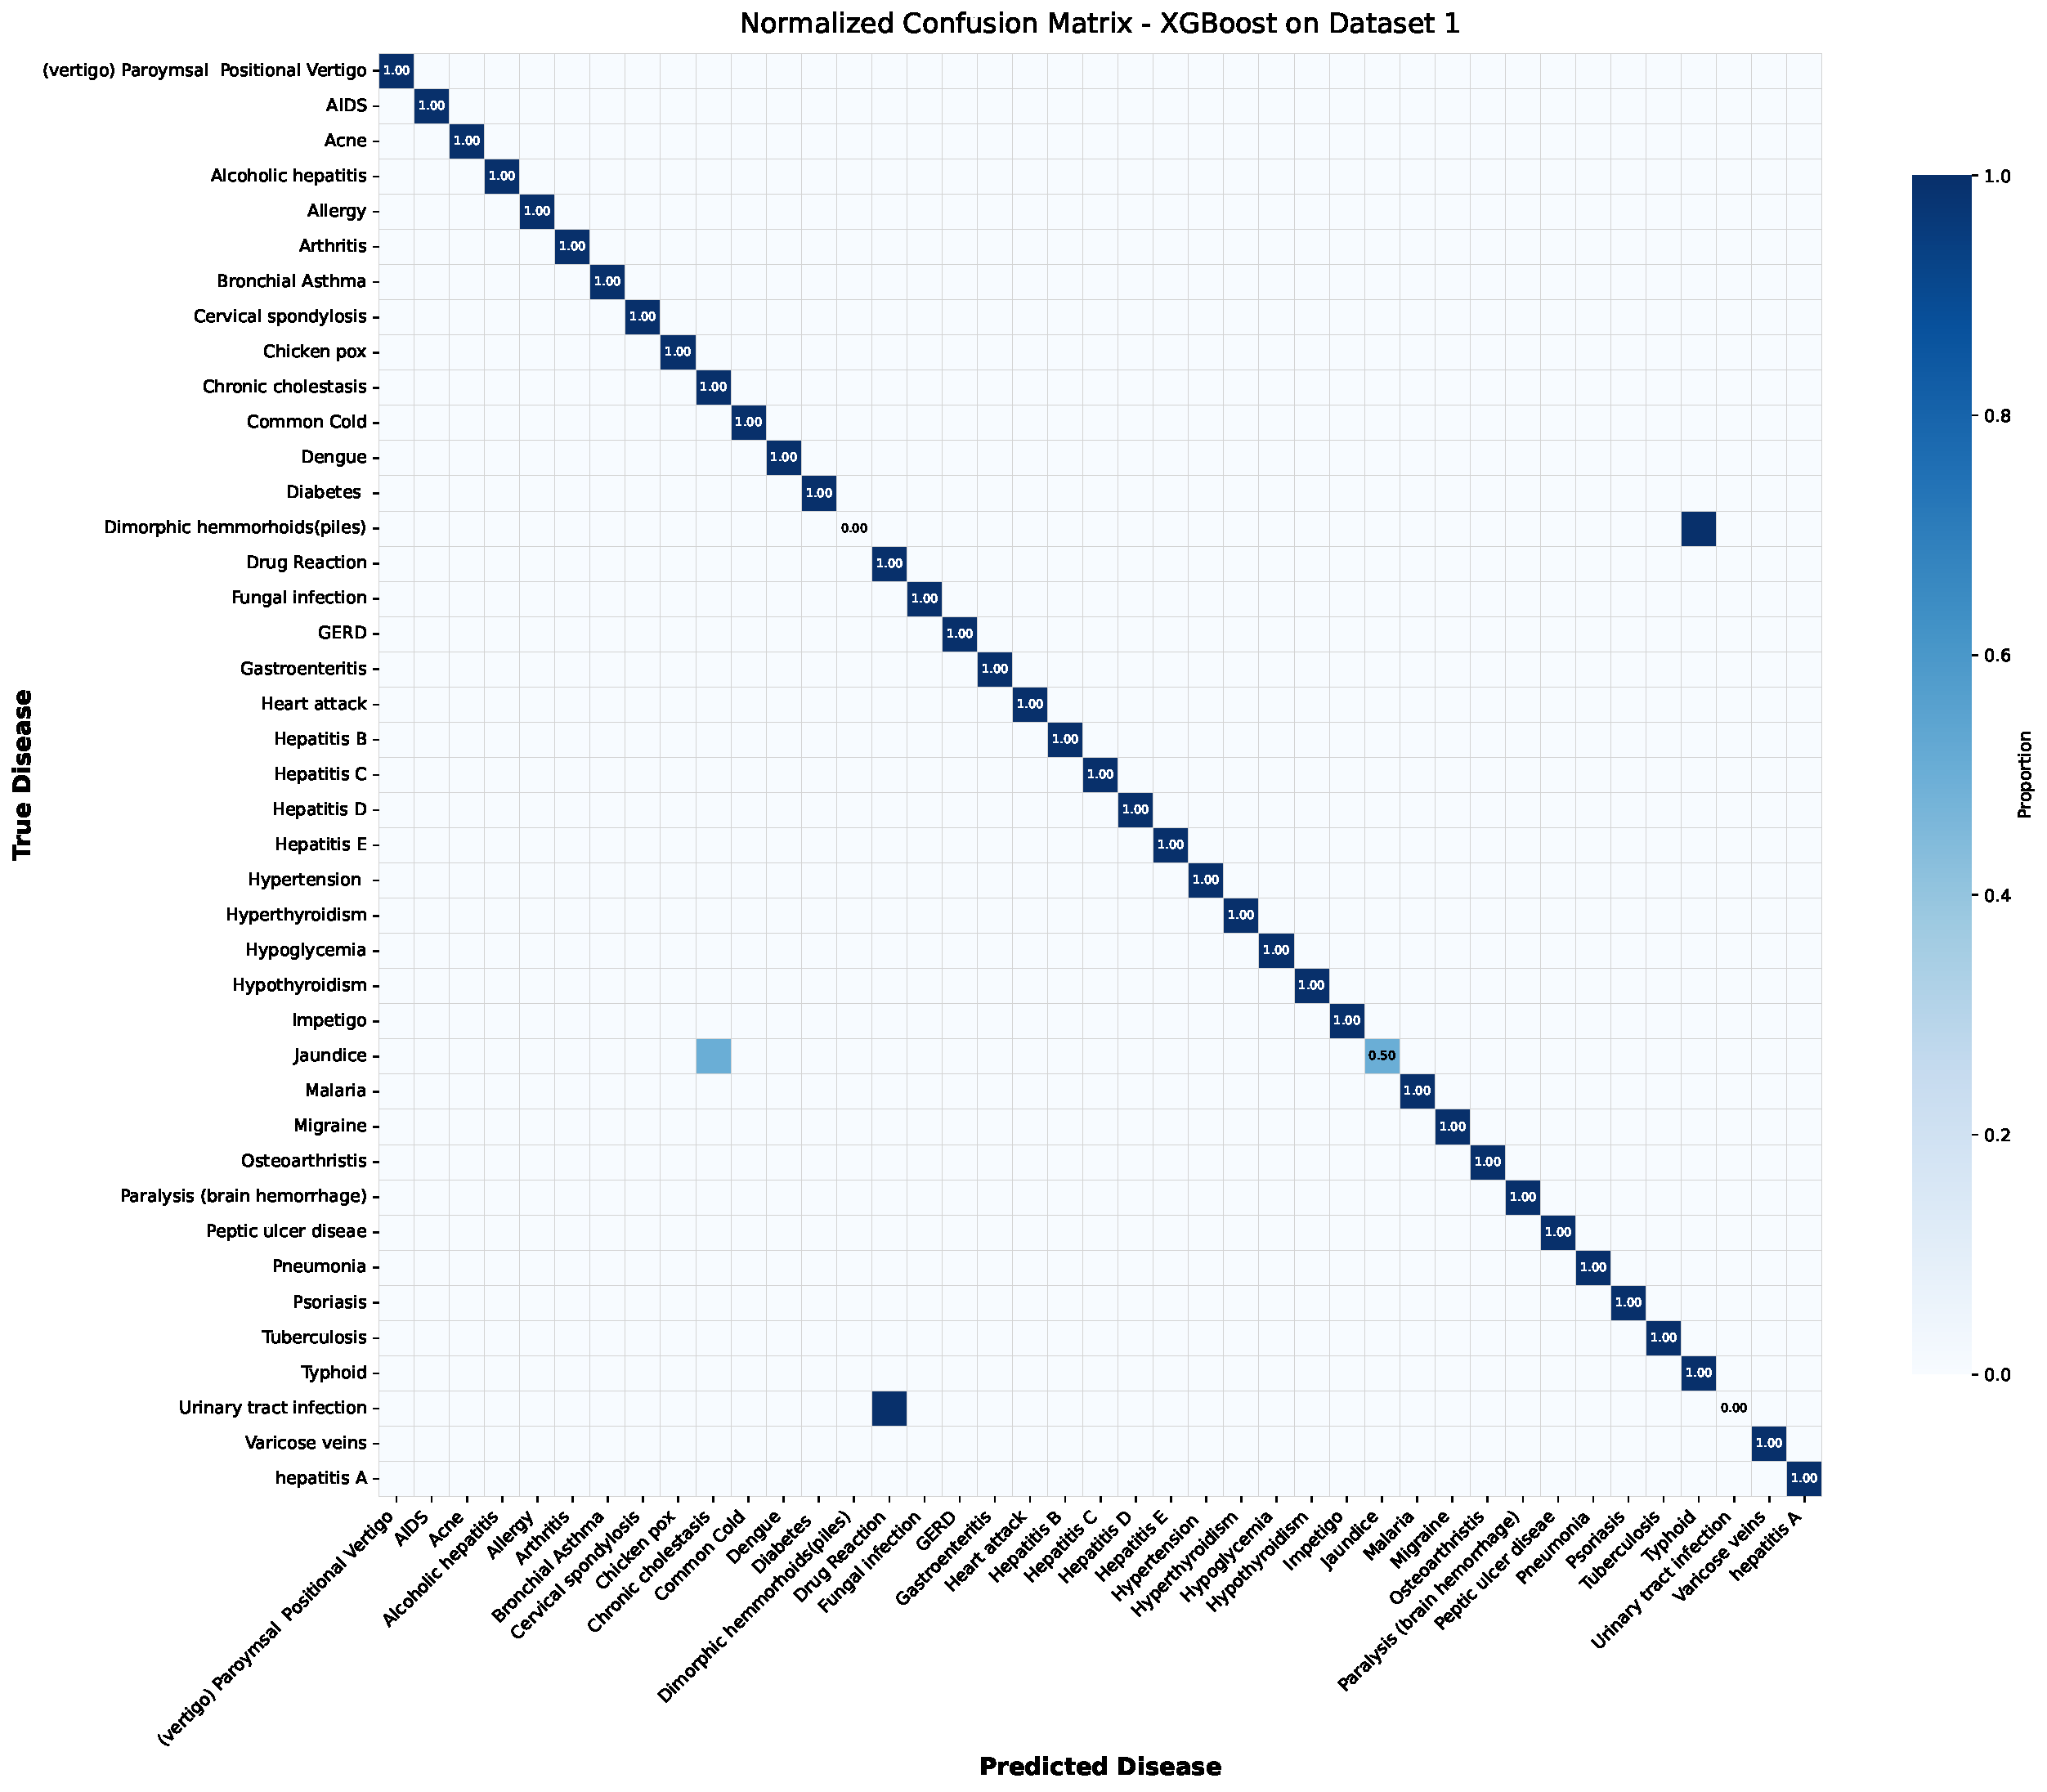
\includegraphics[width=0.85\textwidth]{figures/confusion_matrix.pdf}
\caption{Normalized confusion matrix for XGBoost on Dataset~1. Darker cells on the diagonal indicate correct classifications. Off-diagonal elements show misclassifications.}
\label{fig:confusion_matrix}
\end{figure}

The confusion matrix reveals that the majority of the errors are between diseases with similar symptoms. For instance, related respiratory diseases such as bronchitis and pneumonia were sometimes difficult to distinguish because of similar symptoms like cough, fever, and chest pain. Likewise, various types of skin problems were mixed up when they presented with a similar rash.

Interestingly, some of these confusion pairs are also clinically appropriate, as the diseases commonly have to be managed by the same specialist. A misclassification between two dermatological conditions would still direct the patient to a dermatologist, so the error would not affect the healthcare booking use case.

\section{Feature Importance Analysis}
\label{sec:feature_importance}

Random Forest and XGBoost can be used to calculate feature importances based on the contribution of each feature to the decision-making process. The top 15 most informative symptoms identified by XGBoost on Dataset~1 are shown in Figure~\ref{fig:feature_importance}.

\begin{figure}[H]
\centering
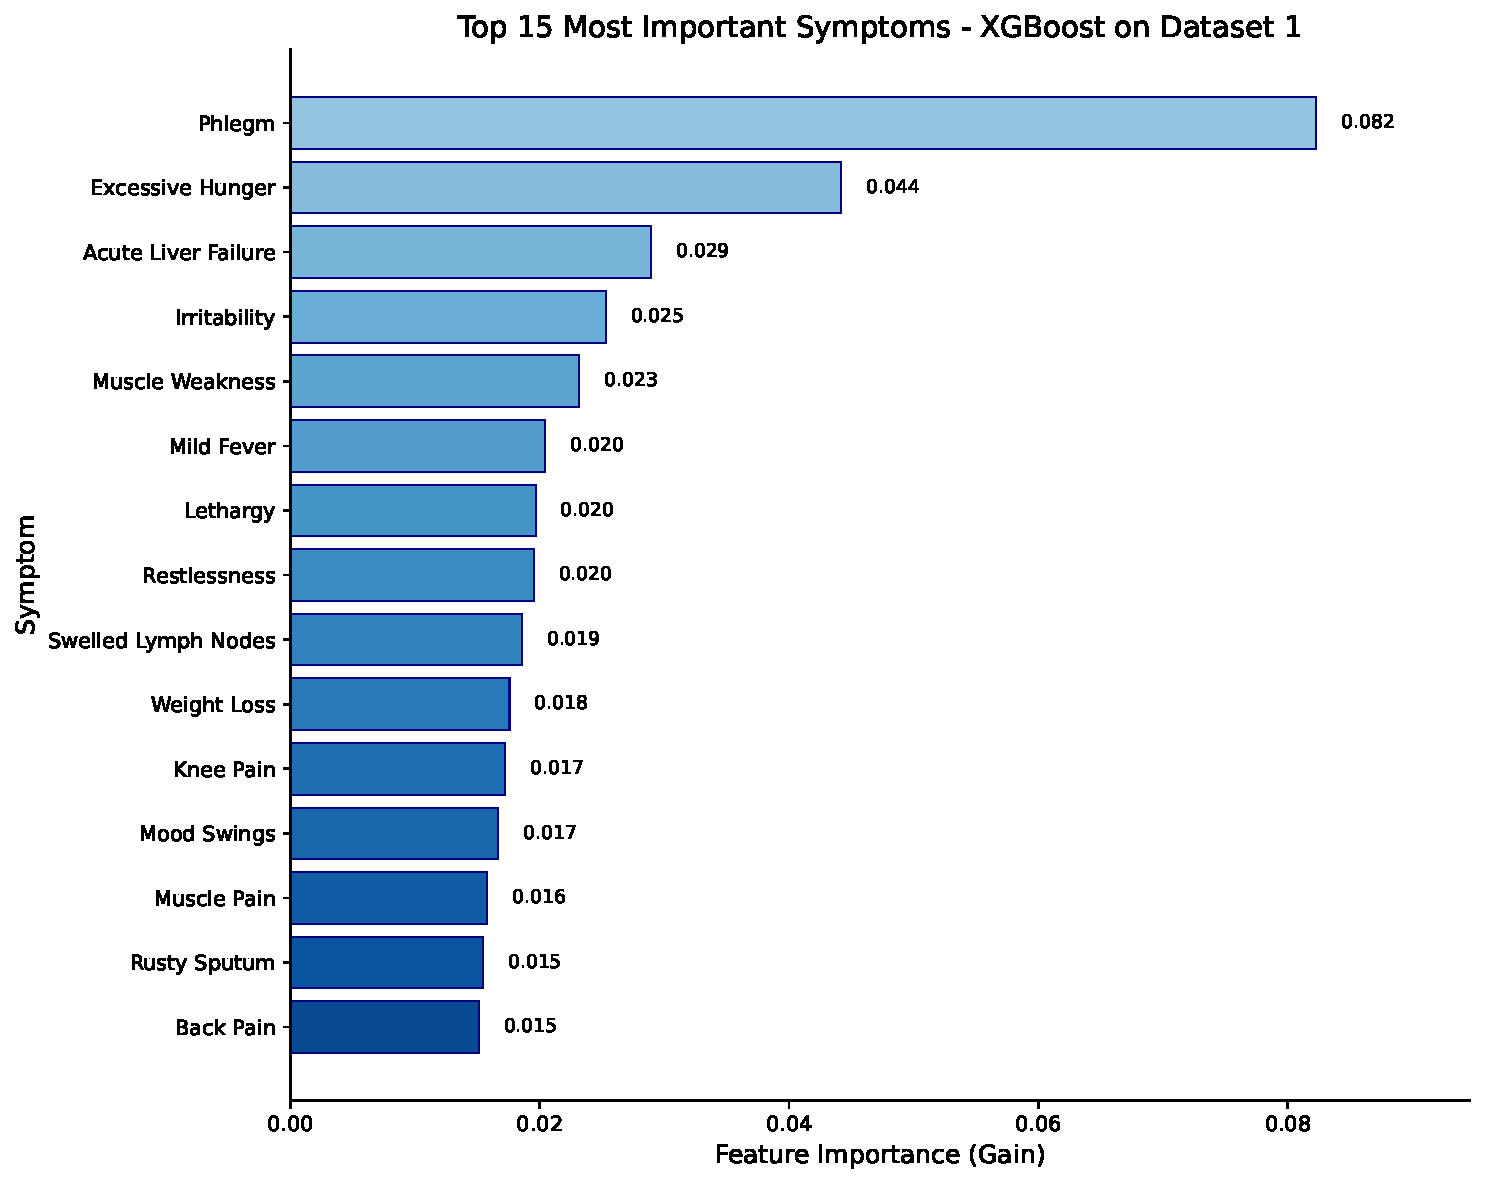
\includegraphics[width=0.85\textwidth]{figures/feature_importance.pdf}
\caption{Top 15 most important symptoms for XGBoost on Dataset~1, ranked by gain-based importance.}
\label{fig:feature_importance}
\end{figure}

The feature importance analysis revealed that certain symptoms provide more information than others. Disease-specific symptoms like ``skin\_rash'', ``chest\_pain'', and ``yellowish\_skin'' were high-ranking. Very general symptoms like fatigue and headache were not so important, as they are found in many diseases and give little discriminating signal.

This indicates that a short symptom questionnaire, consisting of only 15 or 20 carefully selected symptoms, could do as well and be much simpler for patients to complete. A discussion of this possibility is continued in Chapter~\ref{ch:conclusion}.

\chapter{Discussion}
\label{ch:discussion}

This chapter interprets the results, compares the trade-offs between classifiers, acknowledges what this study cannot claim, and discusses the ethical and practical sides of deploying these models.

\section{Interpretation of Results}
\label{sec:interpretation}

After running the experiments, I found that ensemble methods --- Random Forest and XGBoost --- clearly outperformed the three simpler classifiers on both datasets. This makes sense for tabular data with feature interactions: individual trees can learn rules like ``if fever AND rash AND joint pain, predict disease X,'' while a linear model like Logistic Regression cannot represent such conditional patterns without explicit feature engineering.

XGBoost's sequential boosting was particularly helpful for rare diseases. Random Forest can miss rare examples because each tree only sees a bootstrap sample, but XGBoost explicitly focuses each new tree on the mistakes of previous ones. The regularization term in eq.~\ref{eq:xgboost} also helped prevent overfitting on disease categories with few training examples.

All classifiers improved from Dataset~1 to Dataset~2, which confirms what you'd expect from bias-variance theory \citep{Bishop2006}: more data reduces variance. But the benefit was largest for complex models that had room to improve. Naive Bayes hit a ceiling --- its independence assumption limits what it can learn regardless of how much data it sees.

\section{Trade-offs Between Models}
\label{sec:tradeoffs}

Raw performance numbers do not tell the whole story. The choice of classifier for a real deployment depends on several practical factors.

\textbf{Interpretability:} Logistic Regression is the most transparent model. Its coefficients directly show which symptoms push the prediction toward which disease. If a doctor wants to know why the system recommended a dermatologist, Logistic Regression can provide a clear answer. Random Forest and XGBoost offer feature importance rankings but cannot easily explain individual predictions without additional tools like SHAP.

\textbf{Training and prediction speed:} Naive Bayes and Logistic Regression train in seconds even on Dataset~2. SVM was the slowest by a large margin due to its one-vs-one multi-class strategy, which scales poorly with the number of classes. For a mobile health app that needs to update its model frequently, this matters.

\textbf{Handling rare diseases:} XGBoost and Random Forest with class weighting showed the best recall on rare disease classes. Naive Bayes struggled most with imbalanced classes, tending to over-predict common diseases.

\textbf{My recommendation:} For a real healthcare booking system, I would deploy XGBoost or Random Forest as the primary classifier. But I would keep a Logistic Regression model available for when a doctor or regulator asks ``why did the system suggest this specialist?'' --- having an interpretable fallback is worth the slightly lower accuracy.

\section{Limitations and Concerns}
\label{sec:limitations}

This study has several limitations that I want to be upfront about.

\textbf{No external validation.} This is the biggest limitation. I evaluated the classifiers using cross-validation and a held-out test set from the same data distribution. I did not test on an independent clinical dataset. Models that work well on Kaggle data may fail with a different patient population that has different symptom reporting habits or disease prevalence. The accuracy numbers in Chapter~\ref{ch:results} should be treated as optimistic upper bounds.

\textbf{Simplified symptom representation.} The binary encoding doesn't capture severity, duration, or the order symptoms appeared in. A doctor would use all of this. The datasets don't provide it, which limits what the classifiers can learn.

\textbf{Single-disease assumption.} The datasets assign exactly one disease per patient. In reality, patients often have multiple conditions at the same time (comorbidities). A patient with both diabetes and a skin condition would be mishandled by a single-label classifier.

\textbf{No demographic features.} Age, sex, and medical history are important for diagnosis but aren't in either dataset. Adding these would likely improve performance but was outside what the data provided.

\textbf{Hyperparameter search wasn't exhaustive.} I used grid search with predefined ranges. Bayesian optimization or random search over wider ranges might find slightly better configurations, though I doubt this would change the relative ranking of classifiers.

\section{Ethical Considerations}
\label{sec:ethics}

Deploying disease prediction models in healthcare raises issues that go beyond technical performance.

\textbf{Patient safety:} A wrong prediction can lead to a wrong booking. If the model says ``dermatologist'' but the patient actually needs a cardiologist, the delay could be dangerous. Any deployed system must clearly communicate that its predictions are suggestions, not diagnoses, and that seeing a doctor is still necessary.

\textbf{Data protection:} Health data is a special category under the GDPR \citep{GDPR2016}. Processing it requires explicit consent and additional safeguards. A deployed system would need to minimize what data it stores and ensure it is encrypted and access-controlled.

\textbf{EU AI Act:} The recently enacted EU AI Act \citep{EUAI2024} classifies medical AI as high-risk. This means any commercial deployment would require a conformity assessment, risk documentation, human oversight mechanisms, and transparency about how the system works. These are not optional --- they are legal requirements.

\textbf{Bias:} If the training data over-represents certain demographics, the model will perform worse for underrepresented groups. Before deploying this kind of system, fairness audits across age, sex, and ethnicity would be necessary.

\section{Practical Deployment Considerations}
\label{sec:deployment}

Turning these experimental results into a working system involves several steps that are beyond this thesis's scope but worth outlining.

A practical system would present patients with a symptom checklist, encode their selections as a binary vector, run the classifier, and show the predicted disease with a confidence score. The system would then map the disease to the appropriate specialist and suggest available appointment slots.

Not every prediction should be acted on. If the model's confidence is too low, the patient should be directed to a general practitioner instead of a specialist. Setting this threshold means balancing false referrals against missed diagnoses --- a decision that needs medical professionals involved, not just engineers.

Any deployed model would need monitoring. Disease patterns change, new diseases emerge, and the patient population using the system might differ from the training data. Periodic retraining and performance checks would be necessary to catch degradation before it harms patients.

\chapter{Conclusion and Future Work}
\label{ch:conclusion}

\section{Summary of Findings}
\label{sec:summary}

I did a comparison of five machine learning classifiers that predict diseases based on binary symptom vectors: Naive Bayes, Logistic Regression, SVM, Random Forest, and XGBoost. I ran each of them on two Kaggle datasets: one with approximately 5,000 records and one with approximately 246,000 records with the same preprocessing, cross-validation and evaluation processes. The aim was to give a controlled comparison to answer the question: what classifier is most effective to predict disease based on symptoms, and is the answer to this question sensitive to the size of the dataset or skewed class distributions?

The findings indicated that there were distinct performance variations, yet no model performed optimally across all contexts. In Dataset 1, it can be observed that the scores of Logistic Regression and SVM were perfect, and Naive Bayes and Random Forest were also good. Naive Bayes performed the highest accuracy on Dataset~2, and the Logistic Regression and XGBoost also performed well. In general, the optimal model is determined by the size of the dataset, the imbalance of classes, and the accuracy-training-interpretability trade-off.

Logistic Regression was still competitive, as a linear model. It was not as strong on every measure as the best models, yet remains an option when interpretability is valued more than using the final few percentage points of accuracy.

SVM was like Logistic Regression in predictive measures but it was much slower to train especially on the large dataset. One-vs-one multi-class strategy is not that scaled well with the number of classes hence not practical in this application.

Naive Bayes was a powerful baseline and it was particularly competitive on Dataset~2 where it recorded the highest accuracy. It continues to train very fast, thus making it still useful when the simplicity and runtime are more important than the model complexity.

The additional information shifted the image, although not in the same direction. There were models which took advantage of the increased dataset and others failed to become the best overall. This indicates that the actual data should form the basis of model choice when predicting diseases using symptoms, as opposed to making a general assumption that more sophisticated procedures cannot lose.

Error analysis showed that majority of the misclassifications occurred between diseases with similar symptoms. E.g. the various respiratory conditions were often mixed in that they share common symptoms such as cough, fever and chest pain. This is medically explainable and not necessarily an issue to the healthcare booking use case as patients having similar symptom patterns usually require the same kind of specialist anyway.

\section{Contributions}
\label{sec:contributions}

This thesis makes three contributions:

\begin{enumerate}
    \item A comparative evaluation of five classifiers to the same symptom based datasets with the same preprocessing and evaluation setup. The majority of current research experiments one or two classifiers in different settings and this means that comparison between papers cannot be reliable.
    \item A comparison on two datasets, of vastly different size, of the relationship between the performance of classifiers and the availability of data. This is what I could not find in the literature.
    \item An explanation of the steps needed to implement a symptom-based prediction model in a healthcare booking system, both in terms of regulatory obligations pursuant to the EU AI Act and the GDPR.
\end{enumerate}

\section{Recommendations}
\label{sec:recommendations}

According to my discovery, I suggest the following:

\begin{itemize}
    \item Logistic Regression is used when interpretability is important, since the coefficients are simple to interpret and describe.
    \item Use Naive Bayes as a robust and very fast baseline, particularly when there is a constraint on training time or when a simple reference model is required.
    \item XGBoost and Random Forest are helpful tools, and one should not expect them to always be more effective than simpler models on any given dataset.
    \item Instead of SMOTE, use class weighting to deal with the imbalanced classes when features are binary.
    \item Should not be deployed without external validation on actual clinical data, confidence thresholds, and human supervision.
\end{itemize}

\section{Future Work}
\label{sec:future_work}

The thesis will offer a basis on which disease can be predicted through symptoms, yet there are a number of significant directions that where the research can be directed towards in future.

\subsection{Clinical Validation}

The next critical thing is to test these classifiers on actual clinical data. The Kaggle datasets that I have used in this case are helpful in the controlled comparison, but they do not reflect the chaotic nature of the real patient encounters. The actual patients may lose the symptoms, misunderstand questions or give different reports than anticipated. It is quite possible that the disease distribution in an actual clinic is quite different than that in the training data.

It would be possible to collaborate with a hospital or clinic to acquire anonymized patient records, which would enable a much more realistic assessment. This would be based on the gathering of symptom data on real patient experiences (self-reported via a Web form or documented by the nurses at the intake) and the confirmed diagnosis by the doctor. This real-world data could then be trained on by the classifiers and tested on held-out cases.

A study like this would require an institutional review board to approve such a study and would be required to abide by GDPR and other regulations on data protection. It would also have to solve the problem that confirmed diagnoses may not be immediately available --- not all conditions can be diagnosed by lab tests or imaging, which may take days or weeks.

\subsection{Incorporating Additional Features}

The datasets that I employed only have binary symptom data. It is possible that adding patient demographics (age, sex, medical history) as other features would enhance the accuracy of the prediction. Of special importance is age since the prevalence of diseases differs significantly with age. The clinical picture of a rash in a child is not the same as that of the rash in an elderly.

History of medicine is good as well. A patient who has a history of heart disease and presents with chest pain should be diverted as opposed to a healthy 25-year-old reporting the same. Nonetheless, the addition of medical history presents privacy risks and makes the system more complex.

Symptom severity and duration may also be added as another way. The system would not need to binary encode (absent or present), but the patients would be asked to grade the severity on a scale (mild, moderate, severe) and specify the duration that they have had each symptom. It would give the classifier more information and would complicate and lengthen the questionnaire.

\subsection{Multi-Label Classification}

My datasets and methods are based on the assumption that a patient has no more than one disease. In practice, patients are frequently diagnosed with more than one condition (comorbidities). One may either be diabetic and infected with a skin infection, or asthmatic and allergic to seasons. Multi-label classification would enable the model to classify more than one disease of a patient.

This would involve training data in which every patient is classified with all of his or her conditions, not only the primary one. It would also involve changes in the evaluation measures and specialist-mapping logic. Should the model forecast a dermatological condition and a respiratory condition, which specialist should the patient make an appointment with? The system may have to rank according to severity or recommend appointing with several specialists.

\subsection{Specialist Mapping Layer}

I did not apply the disease-to-specialist mapping and concentrated on disease prediction. The creation of this layer would entail medical knowledge of what diseases are referable to which specialists. Certain mappings are self-evident (eczema dermatologist), whereas others are more complicated. A diabetic patient may require an endocrinologist whereas a diabetic patient may require a podiatrist in case of diabetes related foot issues.

The mapping could also rely on the condition severity. A GP may attend to a mild asthma case, whereas a pulmonologist is necessary in a severe case. The addition of severity assessment to the specialist recommendation logic is a promising trend to be pursued in the future.

\subsection{Reduced-Feature Models}

The analysis of feature importance (Section~\ref{sec:feature_importance}) demonstrated that there are symptoms that are far more informative than others. It may be possible to test a reduced-feature model based on only the top 15-20 most important symptoms to determine whether a simpler questionnaire can perform as well. It would make the system much more practical to the patients in case it does.

A 132 yes/no questionnaire is cumbersome and may result in low quality of the data since patients lose concentration. A reduced questionnaire containing 15-20 well selected symptoms would be easy to fill in and may even enhance the quality of data by minimizing the probability of patients selecting the questions by mistake or by clicking the questions randomly.

The issue is which symptoms should be retained. The rankings of the feature importance are global (average of all diseases), and some of the symptoms may be important in particular diseases, though they are not important in all diseases. It would require a careful analysis to identify a subset of the symptoms that would be well covered in all disease categories.

\subsection{Ensemble Methods and Model Stacking}

Another interesting direction is to combine several classifiers instead of choosing one. An example would be XGBoost as the main model, but when XGBoost and Logistic Regression disagree with one another on a prediction, this may indicate uncertainty, and the patient may be referred to a GP rather than a specialist.

More advanced ensemble techniques such as stacking (training a meta-model that takes the predictions of several base models) may theoretically be even more effective. This, however, complicates the system and makes it more difficult to interpret and maintain.

\subsection{Active Learning and Adaptive Questionnaires}

An adaptive questionnaire may provide follow-up questions based on the responses given earlier instead of questioning each patient on all 132 questions to assess their symptoms. As an example, when a patient presents with a rash, the system may ask questions related to the skin issue (itching, location, duration) but not irrelevant symptoms.

This would reduce the length of the questionnaire and make it more individualized, however, it would complicate the representation of the features and would necessitate an alternative form of modeling, which may be a decision tree or reinforcement learning.

\subsection{Deployment and Monitoring}

Lastly, the construction and implementation of a full system would entail all of the pragmatic aspects covered in Section~\ref{sec:deployment}: the need to integrate with appointment scheduling systems, confidence thresholds, edge cases, and performance monitoring. A pilot implementation in a small clinic or a university health center would be informative as to what works and what does not work in practice.

% --- Acknowledgements ---
\chapter*{Acknowledgements}
\addcontentsline{toc}{chapter}{Acknowledgements}

% TODO: 100-150 words


% --- Bibliography ---
\bibliographystyle{apalike}
\bibliography{references}

% --- Appendix ---
\begin{appendices}
\chapter{Supplementary Materials}
\label{app:supplementary}

% TODO: Preprocessing pipeline details, Table A1 (hyperparameters), software versions

\end{appendices}

\end{document}
